\documentclass[twocolumn]{aastex631}
\received{\today}
\shorttitle{NEOCP in Era of LSST}
\graphicspath{{figures/}}

\usepackage{lipsum}
\usepackage{physics}
\usepackage{multirow}
\usepackage{xspace}
\usepackage{natbib}
\usepackage{fontawesome5}
\usepackage{xcolor}
\usepackage{wrapfig}
\usepackage[figuresright]{rotating}

% remove indents in footnotes
\usepackage[hang,flushmargin]{footmisc} 

\newcommand{\todo}[1]{{\color{red}{[TODO: #1}]}}
\newcommand{\needcite}{{\color{magenta}{(needs citation)}}}
\newcommand{\placeholder}[1]{{\color{gray} \lipsum[#1]}}

% for shorthand/consistency
\newcommand{\dig}{\texttt{digest2}}
\newcommand{\sss}{S3M}
\newcommand{\mpco}{MPCORB}

% custom function for adding units
\makeatletter
\newcommand{\unit}[1]{%
    \,\mathrm{#1}\checknextarg}
\newcommand{\checknextarg}{\@ifnextchar\bgroup{\gobblenextarg}{}}
\newcommand{\gobblenextarg}[1]{\,\mathrm{#1}\@ifnextchar\bgroup{\gobblenextarg}{}}
\makeatother

\begin{document}

\title{{\Large The Sky is Falling?}\\The NEOCP in the Era of LSST}

% affiliations
\newcommand{\UW}{Department of Astronomy, University of Washington, Seattle, WA, 98195}

\author[0000-0001-6147-5761]{T. Wagg}
\affiliation{\UW}

\author[0000-0003-1996-9252]{M. Juric}
\affiliation{\UW}

\author{\dots more}

\correspondingauthor{Tom Wagg}
\email{tomjwagg@gmail.com}

\begin{abstract}
    \todo{}
    \placeholder{1}

    \placeholder{2}
\end{abstract}

\keywords{Near-Earth objects, Asteroids, Solar system, Small Solar System bodies, Surveys}

\section{Introduction} \label{sec:intro}
Near-Earth Objects (NEOs) are objects that may come close enough to the Earth that small perturbations in their orbit lead to a collision course. A simple definition for NEOs is that there are small solar system bodies that have a perihelion less than $1.3 \unit{AU}$ \citep[e.g.][]{Jones+2018}. Given the threat posed by these objects, it is therefore critical that we catalogue and determine the orbit of NEOs.

The Minor Planet Center maintains a catalogue of known NEOs and their orbits\footnote{\url{https://www.minorplanetcenter.net/iau/MPCORB/NEA.txt}}, as well as the NEO confirmation page (NEOCP\footnote{\url{https://www.minorplanetcenter.net/iau/NEO/toconfirm_tabular.html}}), which lists potential NEOs that should be prioritised for additional observations by the NEO follow-up community. An object is only listed on the NEOCP when it has a high probability of being an NEO. This probability is quantified using the \dig{} code, which assigns a score between 0 and 100 and only objects with a score of 65 or more are listed on the page \citep{Keys+2019}. Currently, on average around two dozen objects are added to the NEOCP on each night.

The Legacy Survey of Space and Time (LSST) will rapidly increase the rate at which NEOs are discovered and sent to the NEOCP. \todo{need more details} \placeholder{1}

Given this increased discovery rate, if LSST operates in the same way as current telescopes that work on NEO discovery, the number of objects submitted to the NEOCP will increase by several orders of magnitude. This will make it difficult for the follow-up community to prioritise particular objects and may lead to some objects being missed. However, many of the objects that LSST observes will be re-observed and discovered by LSST alone, though there will still be a sizeable fraction of objects that require community follow-up. It is therefore important to identify this fraction so that the follow-up community can effectively prioritise observations.

This paper quantifies the impact of LSST on the NEOCP and the fraction of objects that require community follow-up.

Our paper is structured as follows. In Section~\ref{sec:method}, we describe the methods for simulating LSST observations, calculating \dig{} scores for the NEOCP and our algorithm for predicting whether LSST will detect an object based on a single night of observations. In Section~\ref{sec:results}, we present our findings for the total number and type of objects submitted to the NEOCP by LSST. Based on these results, in Section~\ref{sec:discussion} we present recommendations for how objects should be submitted to the NEOCP from LSST. We conclude in Section~\ref{sec:conclusion}.

\section{Method} \label{sec:method}
In order to make predictions for the NEOCP in the era of LSST, we make simulated observations of a catalogue of solar system objects that takes into account currently known objects. We then use the \dig{} code to calculate NEO scores for each object and use these values to make predictions for the NEOCP. Additionally, we present an algorithm for predicting whether LSST will detect an object given a single night of observations. In the subsections below we explain each of these steps in more details.

\subsection{Simulated Observations}

In order to investigate the effect of LSST sources on the NEOCP, we use a `hybrid' solar system object catalogue. This catalogue contains both real and synthetic objects, whilst retaining the same overall distributions in position, velocity and absolute magnitude found in the purely synthetic catalogue (see Appendix~\ref{app:hybrid}).

We perform mock LSST observations using a baseline v2.1 10 year \texttt{OpSim} simulation \citep{Bianco+2022}. These observations account for both scheduled and unscheduled downtime and simulate the current baseline observing strategy that will be followed by LSST. \todo{Mario should check this (and the citation)}

\subsection{\dig{} Score Calculation}\label{sec:digest2_score}
The main criterion for an object to be placed on the NEOCP is for it to receive an NEO score of at least 65. This score from 0 to 100 assesses the probability that the object is an NEO and is calculated using the \dig{} code \citep{Keys+2019}. We therefore use the same code to check which of the simulated observations of the hybrid catalogue could be submitted to the NEOCP.

We use \dig{} to calculate the NEO score of each NEO and MBA in the hybrid catalogue that is observed in the first year. We apply three further cuts before considering which submissions are eligible for the NEOCP \needcite{}.
\begin{enumerate}
    \item \textbf{Number of observations:} We consider only objects which have at least 2 observations on a given night (though we investigate the effect of making this limit more stringent - see Section.~\ref{sec:traffic_basic})
    \item \textbf{Minimum arc length:} We ensure that each arc is at least 1 arcsecond in length
    \item \textbf{Maximum time separation:} We set the maximum time between observations to 90 minutes. Thus we only allow tracklets that have at least one pair of observations that occur within 90 minutes of each other
\end{enumerate}

In Figure~\ref{fig:digest2_example} we show the distribution of \dig{} scores for the NEOs and MBAs in the first year of observations. As expected most NEOs have scores around 100 and most MBAs have scores around 0. However, we highlight that due to the volume of MBAs, the \dig{} score does not perform well in classifying NEOs. In particular, even an object assigned a score of 100 only has around a 3\% chance of actually being an NEO. \todo{not sure if this is right place}

\begin{figure}
    \centering
    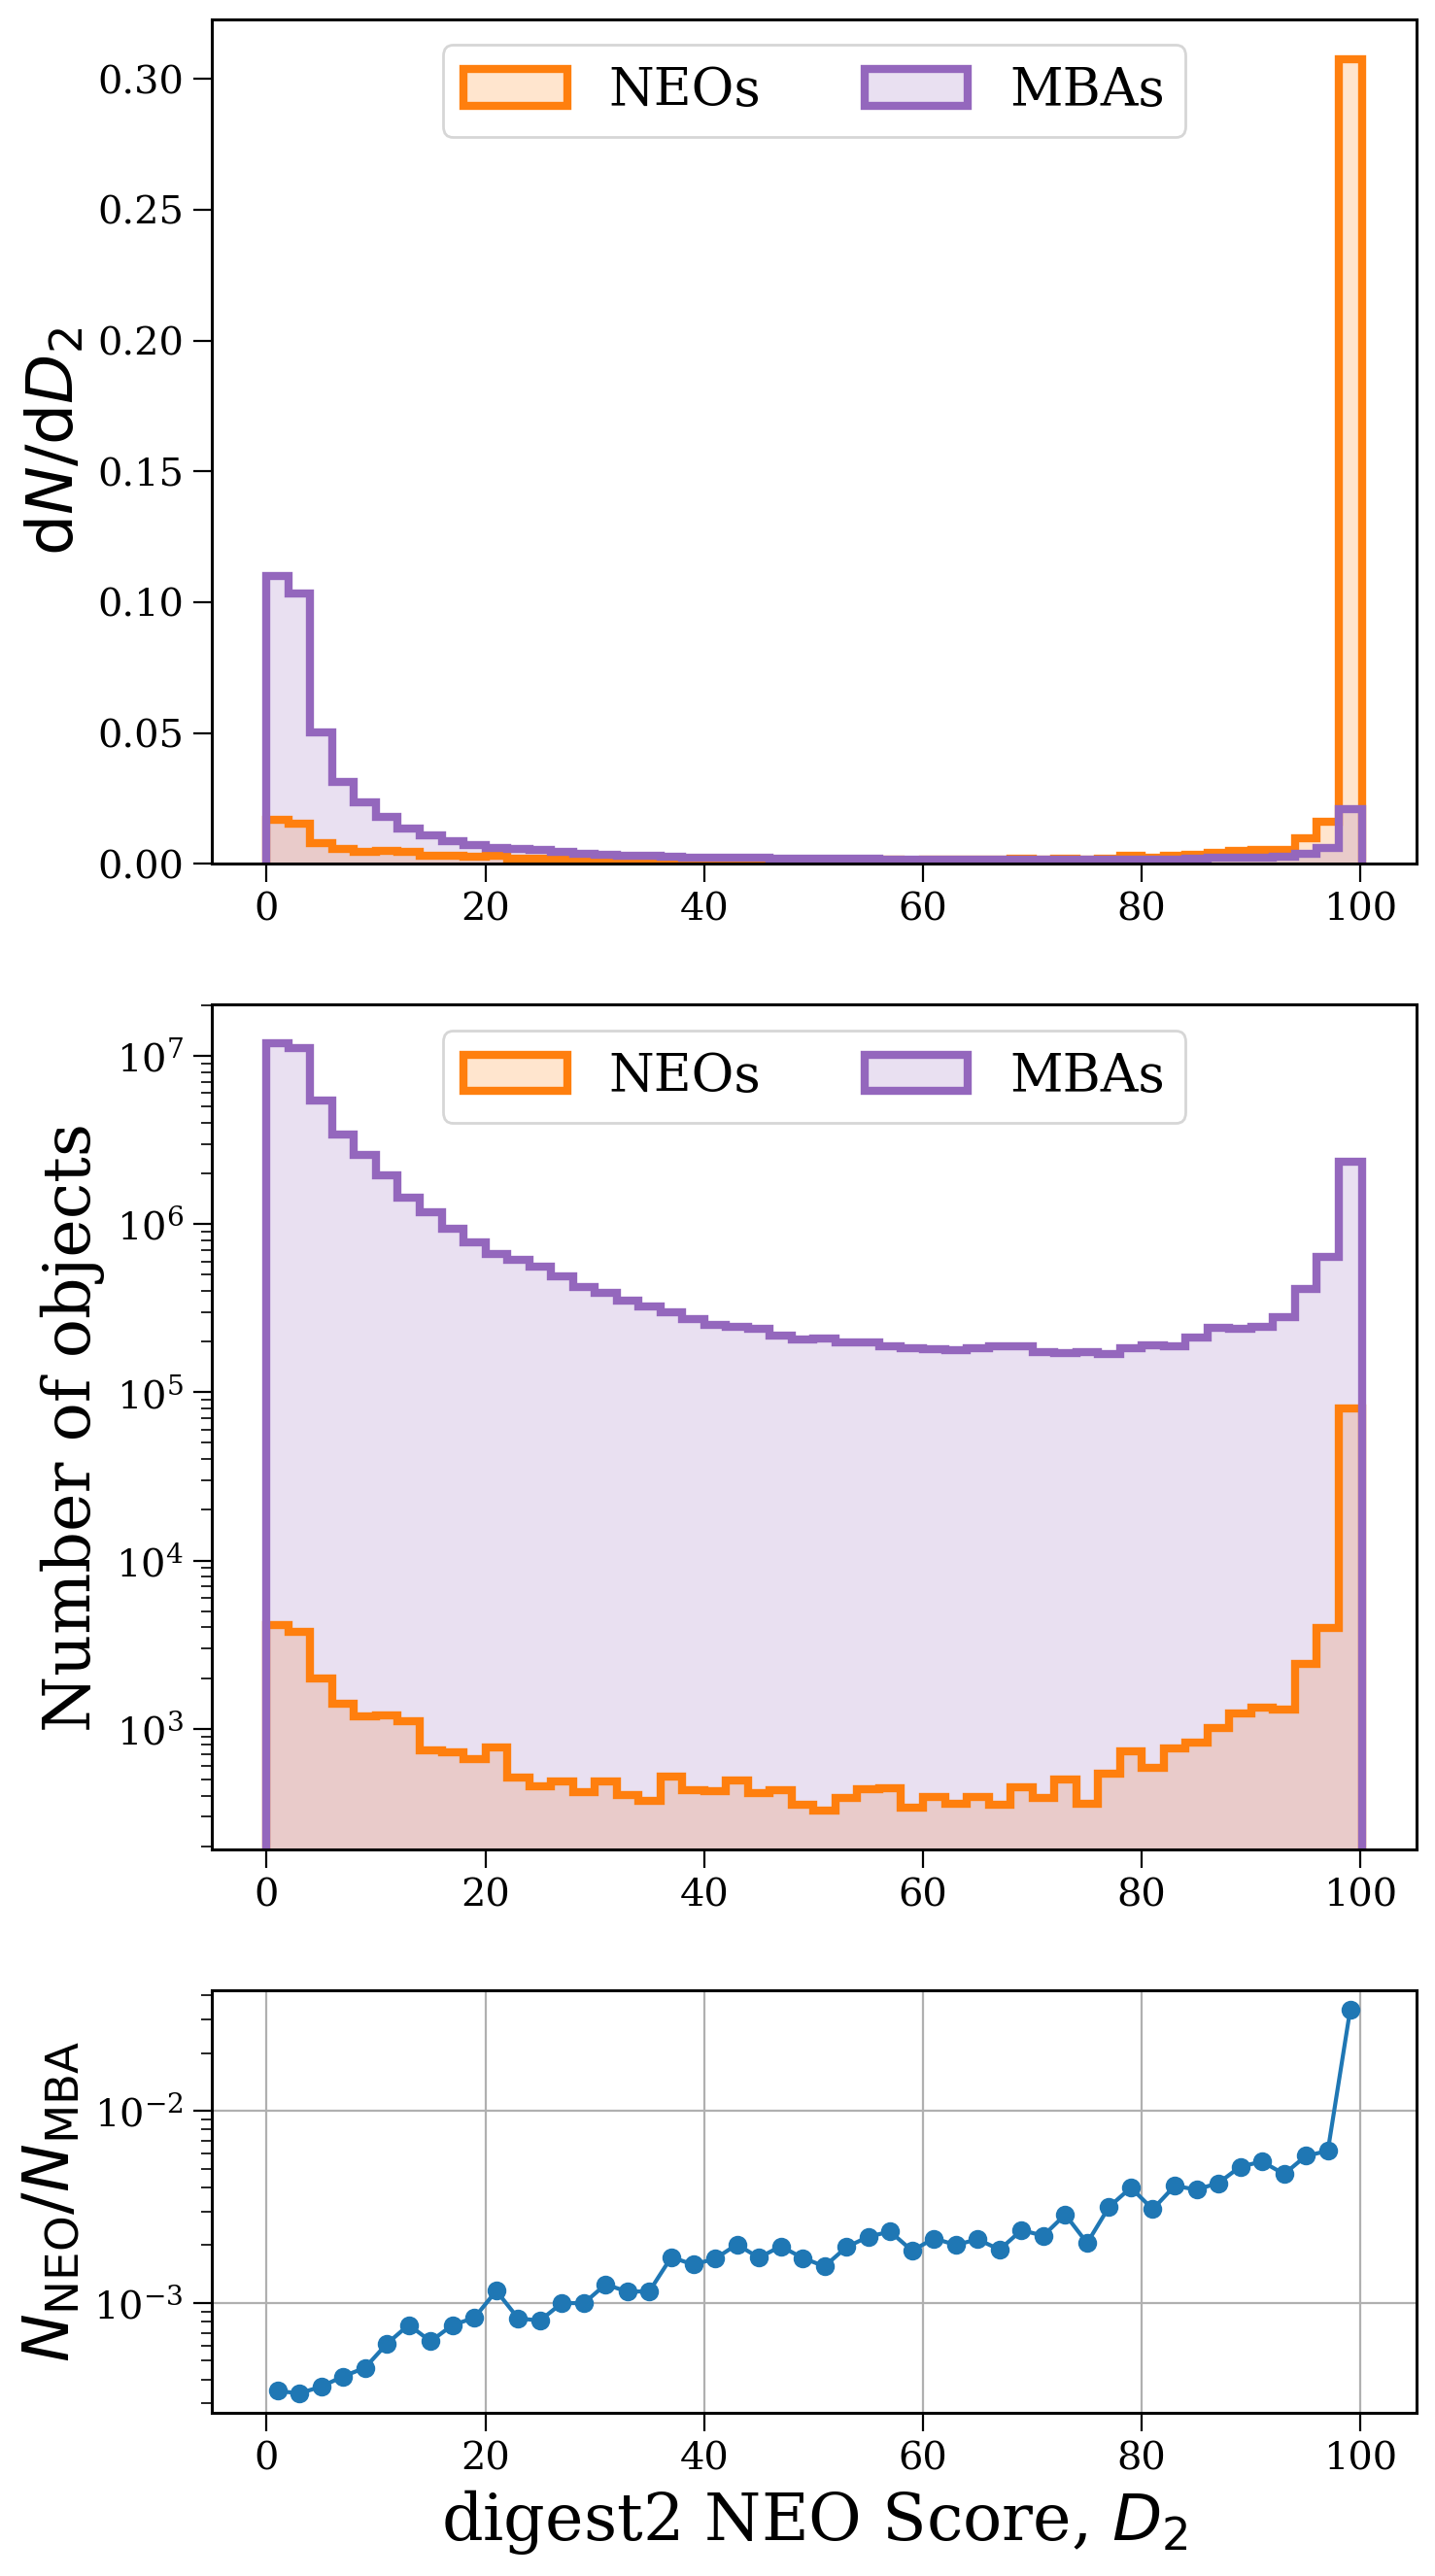
\includegraphics[width=\columnwidth]{digest2_pollution.png}
    \caption{\dig{} scores for all NEOs and MBAs observed in the first year of our simulated LSST observations. The top panel shows normalised histograms, the middle panel shows un-normalised histograms and the final panel shows the ratio of the histogram in the middle panel. Note that the latter two panels are on a logarithmic scale.}
    \label{fig:digest2_example}
\end{figure}

\subsection{Estimating LSST Detection Probability}\label{sec:pred_alg}
\begin{figure*}[htb]
    \centering
    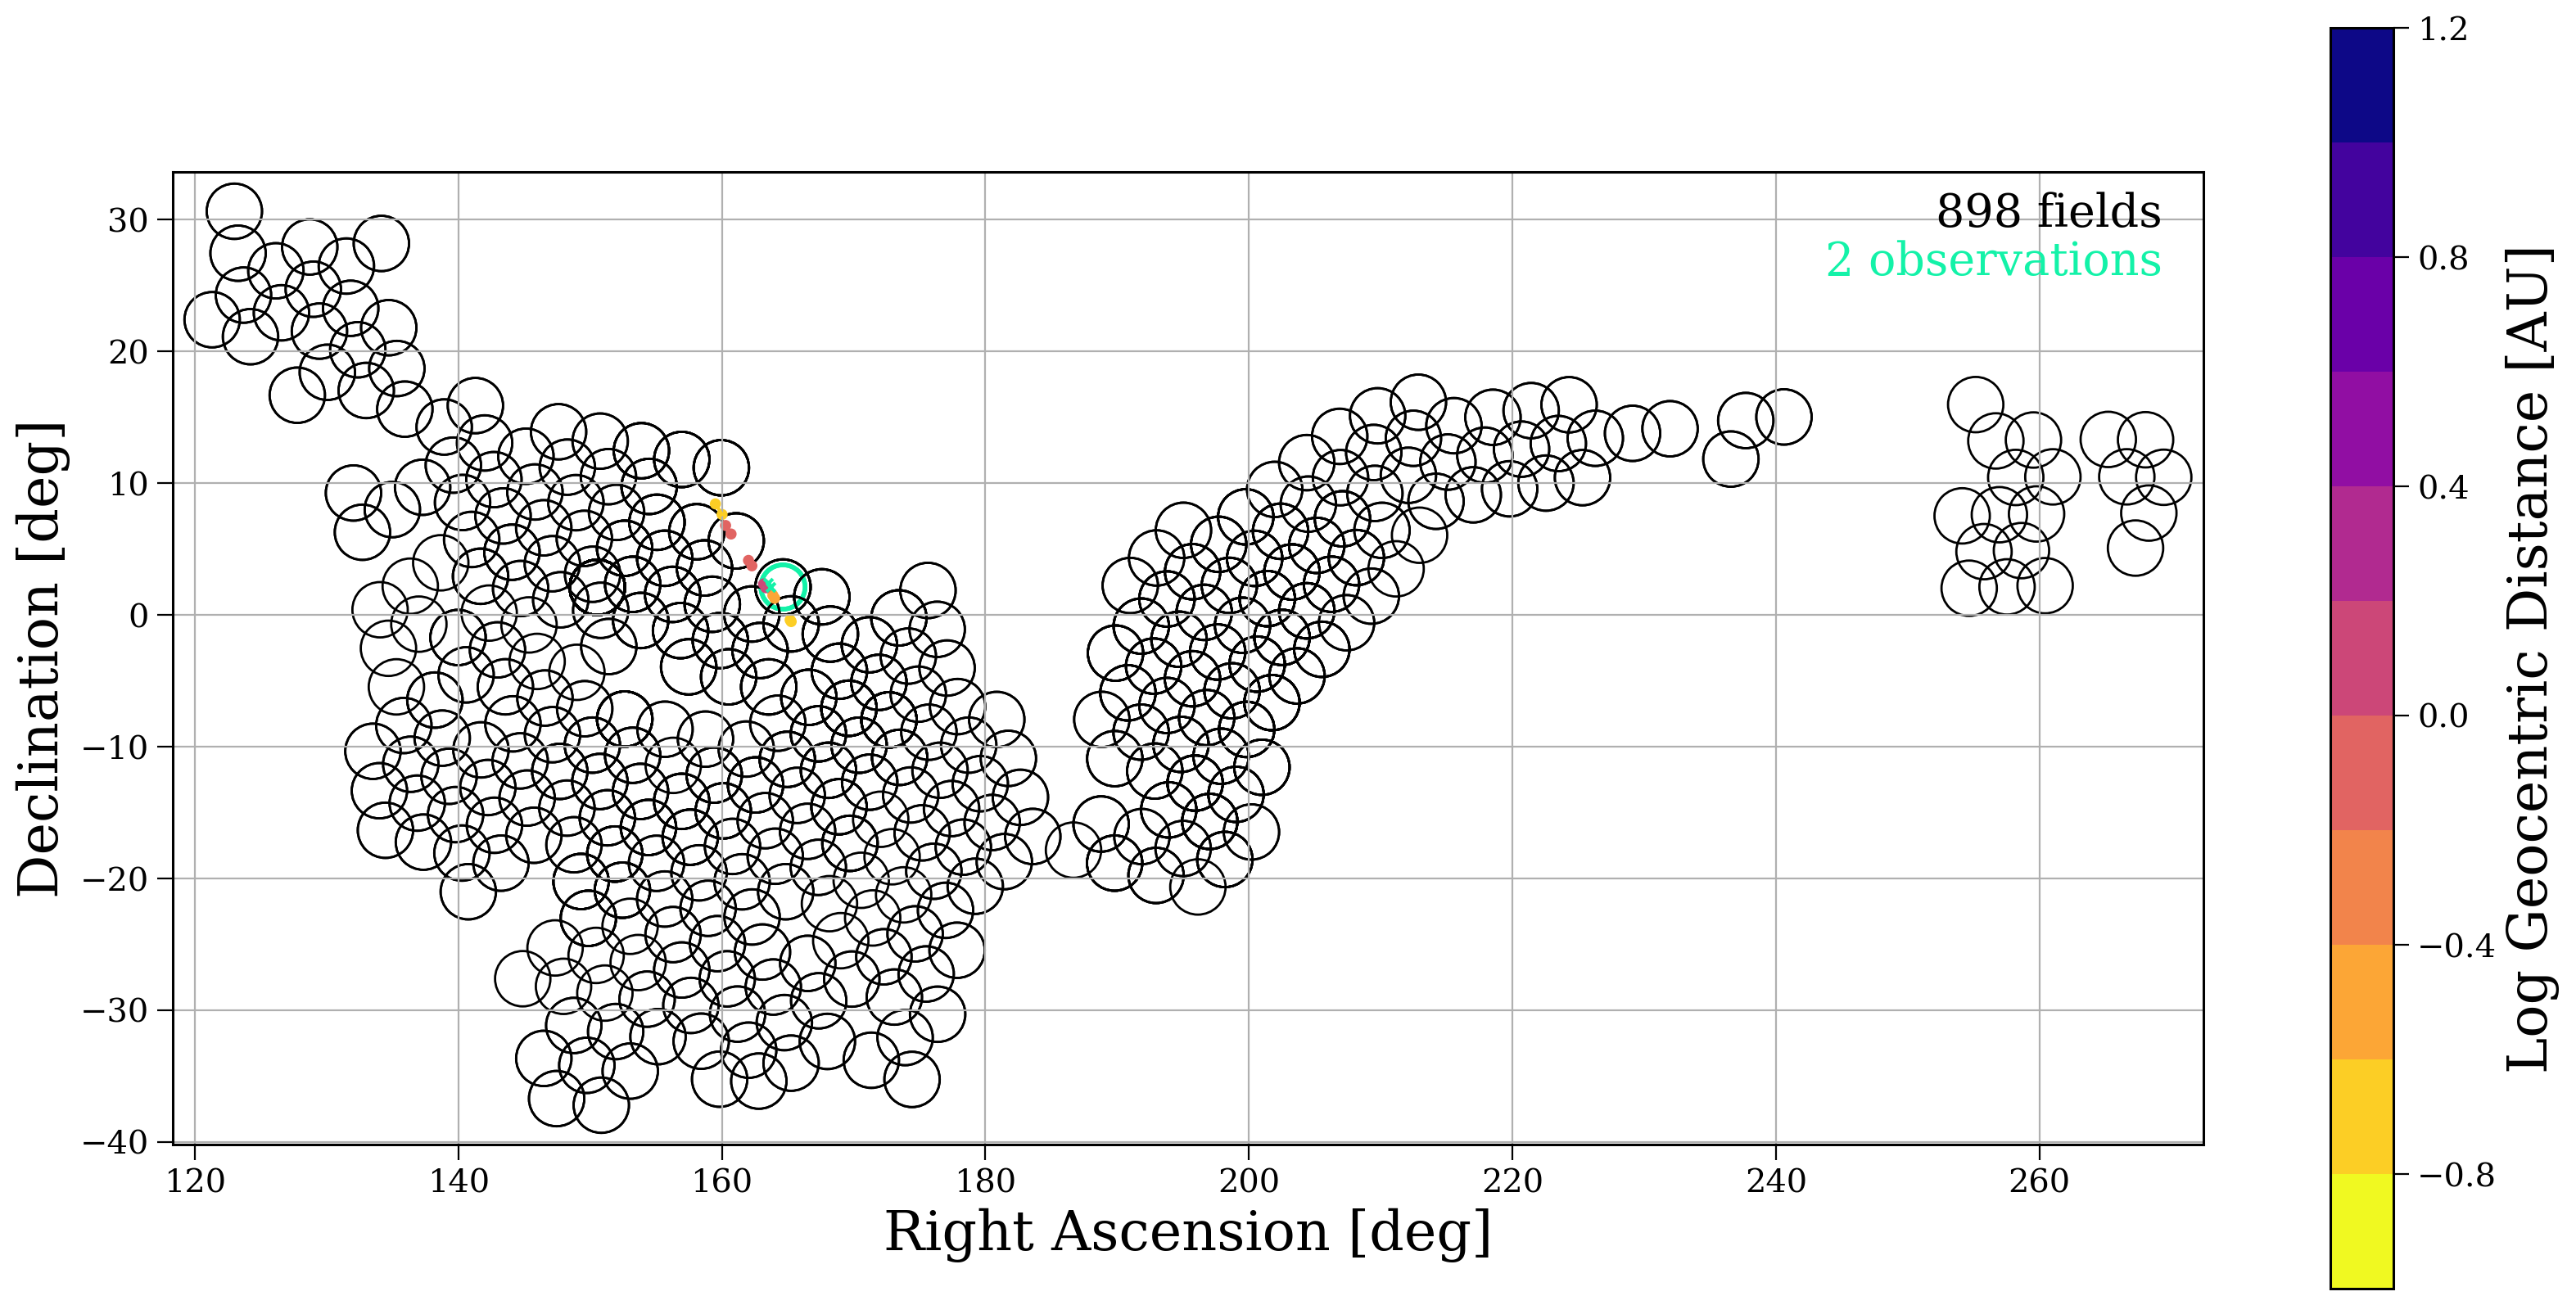
\includegraphics[width=\textwidth]{methods_placeholder.png}
    \caption{A demonstration of the LSST detection probability prediction. Black circles (to scale with $2.1^{\circ}$ radii) represent a bounding circle of LSST's camera footprint for each visit in this night's predicted schedule. For each orbit we plot the object's predicted location at the start and end of the night and colour them by the assumed distance. In cyan we show true position of the object and outline any visits that produce an observation in cyan also.}
    \label{fig:circles}
\end{figure*}

In choosing which objects to submit to the NEOCP from LSST, it also important to consider whether the object would be detected by LSST without external follow-up. We therefore propose a method of \textit{predicting} whether an observed object will be detected by LSST based on current observations. This requires one to predict both the location and magnitude of the object on subsequent nights, as well as the visit schedule of LSST.

In order to determine the location of an object on the following nights one needs to know its orbit. Each object on a given night consists of at least two observations, $O$, that have the form
\begin{equation}
    O = \{ \alpha, \delta, t \}
\end{equation}
where $\alpha$ is the right ascension, $\delta$ is the declination and $t$ is the time of observation. One can then determine the proper motion of the object on the sky, ($\dot{\alpha}$, $\dot{\delta}$), by calculating the change in position over time between the two observations. This determines 4 and the 6 orbital elements, but the topocentric distance, $D$ and radial velocity, $\dot{D}$ of the object are unconstrained.

We draw a sample of $D$ uniformly in log-space between $[0.1, 10] \unit{AU}$ and a sample of $\dot{D}$ uniformly between $[-50, 10] \unit{km}{s^{-1}}$ to create a grid of $(D, \dot{D})$. Combining these with the measured $(\alpha, \delta, \dot{\alpha}, \dot{\delta})$ values (and adding $0.1^{\prime\prime}$ of scatter to the measured on-sky positions to account for the detector uncertainty), we create a series of possible variant orbits for the object and adjust them to account for the light travel time using \texttt{THOR} \citep{Moeyens+2021}. Since we are only interested in NEOs, we mask out any orbits that have a perihelion distance of greater than $1.3 \unit{AU}$. Additionally, we determine the absolute magnitude of the object for each orbit using the HG-system. We convert the apparent magnitudes of the observations in the first night to V-band magnitudes using the LSST colour definitions, assuming a C-type asteroid \citep{Jones+2018}. We then use the mean observed V-band magnitude, the assumed distances and a fixed slope parameter of $G = 0.15$ \needcite{} to calculate the current absolute magnitude.

Finally, using \texttt{OpenOrb}, we produce ephemerides for the orbits for each visit in the following 14 nights of the predicted schedule that the object could potentially reach based on its observed on-sky motion \citep{Granvik+2009}. For each orbit and each field, we check whether the object is within the LSST camera footprint of the field using \texttt{rubin\_sim}\footnote{\url{https://github.com/lsst/rubin\_sim}}. We additionally convert the predicted apparent magnitude back to the relevant filter and assess whether the object has an apparent magnitude brighter than the $5\sigma$ depth of field. If both of these criteria are met then we assume an observation has been made. We show an example of the predictions produced by this method in Fig.~\ref{fig:circles}

Each orbit is defined as producing a detection if it has at least 3 observations on at least 3 nights in a 15 day window, requiring that the minimum arc length is 1 arcsecond and that the maxmimum separation between observations is 90 minutes. We additionally account for all prior observations in this calculation. For example, if we were determining the probability of detection for an object that is observed on night 10 and has previously been observed on night 8, even if we only predict that it will be observed on night 14 in the next 15 days, this would still be deemed a detection. We estimate the overall probability of the object being detected by LSST as a simple fraction of orbits that produce detections.

\section{Results} \label{sec:results}
\subsection{Traffic and Purity of the NEOCP}\label{sec:traffic_basic}
\begin{figure*}
    \centering
    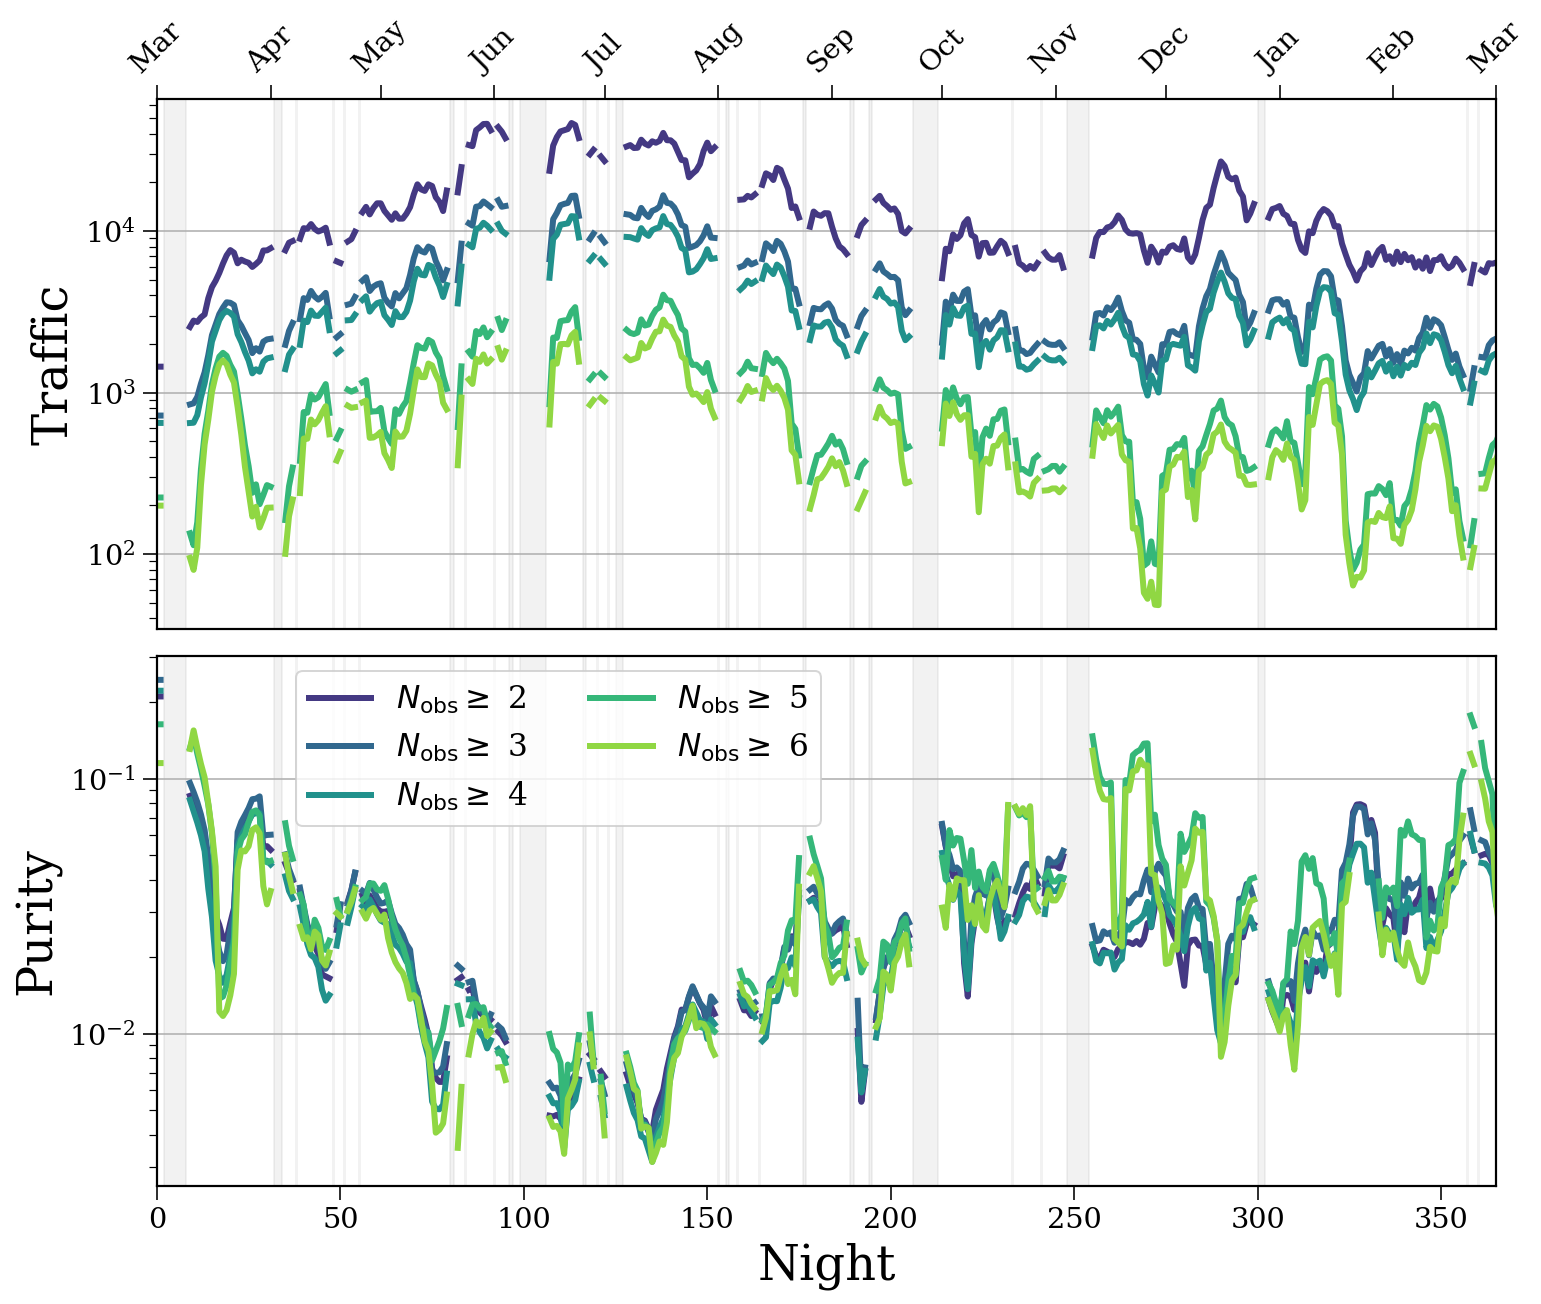
\includegraphics[width=\textwidth]{traffic_purity.png}
    \caption{Traffic (number of objects sent) and purity (fraction of objects sent that are NEOs) of the NEOCP during the first year of LSST if every observation that qualifies for submission is submitted. Each line is plotted using a rolling window of a week to smooth stochastic effects. Different lines correspond to different constraints on the number of observations for a tracklet to be submitted. Nights on which no observations were taken are highlighted with grey areas.}
    \label{fig:neocp_traffic}
\end{figure*}

In Figure~\ref{fig:neocp_traffic}, we summarise the effect that LSST submissions would have on the NEOCP if \textit{every} object that met the \dig{} score criterion was submitted. The top panel shows the traffic of the NEOCP, meaning the number of objects that would be submitted to the page, whilst the bottom panel shows the purity, meaning the fraction of objects submitted to the page that are actually NEOs.

The current typical traffic of the NEOCP is on the order of two dozen new submissions per night. We show in the top panel that this traffic would increase by up to 3 orders of magnitude as a result of LSST submissions. Each line corresponding to a different number of minimum nightly observations (increasing from the original choice of 2 as discussed in Section~\ref{sec:digest2_score}). Although the traffic is lower when requiring more observations, even with a minimum of 6 observations the traffic can reach several thousands of submissions per night, which is far more than the NEOCP is currently equipped to handle.

The purity of the NEOCP is also severely impacted by LSST observations, with the abundance of MBA observations polluting the page as false NEOs. For almost the entire year the page will have a purity below 10\%, meaning that only 1 in 10 objects on the page is actually an NEO. This can decrease below even 1\% and thus a lot of follow up time would be wasted in looking at MBAs masquerading as NEOs.

There are two periodic effects that can be noted in both the traffic and the purity panels. There is a clear seasonal variation over the year as the ecliptic plane moves through the sky. LSST observes from the southern hemisphere and thus in first half of the year when the ecliptic is at lower declinations, more MBAs will be observed. This both increases the traffic and decreases the purity of the NEOCP. In addition to this long term variation, there are also shorter term variations that are most clearly seen in the purity panel. On day 17 and approximately every 30 days after this there is a periodic decrease in the purity of the page. This coincides with the occurrence of a full moon, since LSST has to observe a different part of the sky during this time and this leads to more MBA detections and thus lower purity.

\todo{Check that I explained both of these effects correctly (particularly the moon one)}

\begin{figure*}
    \centering
    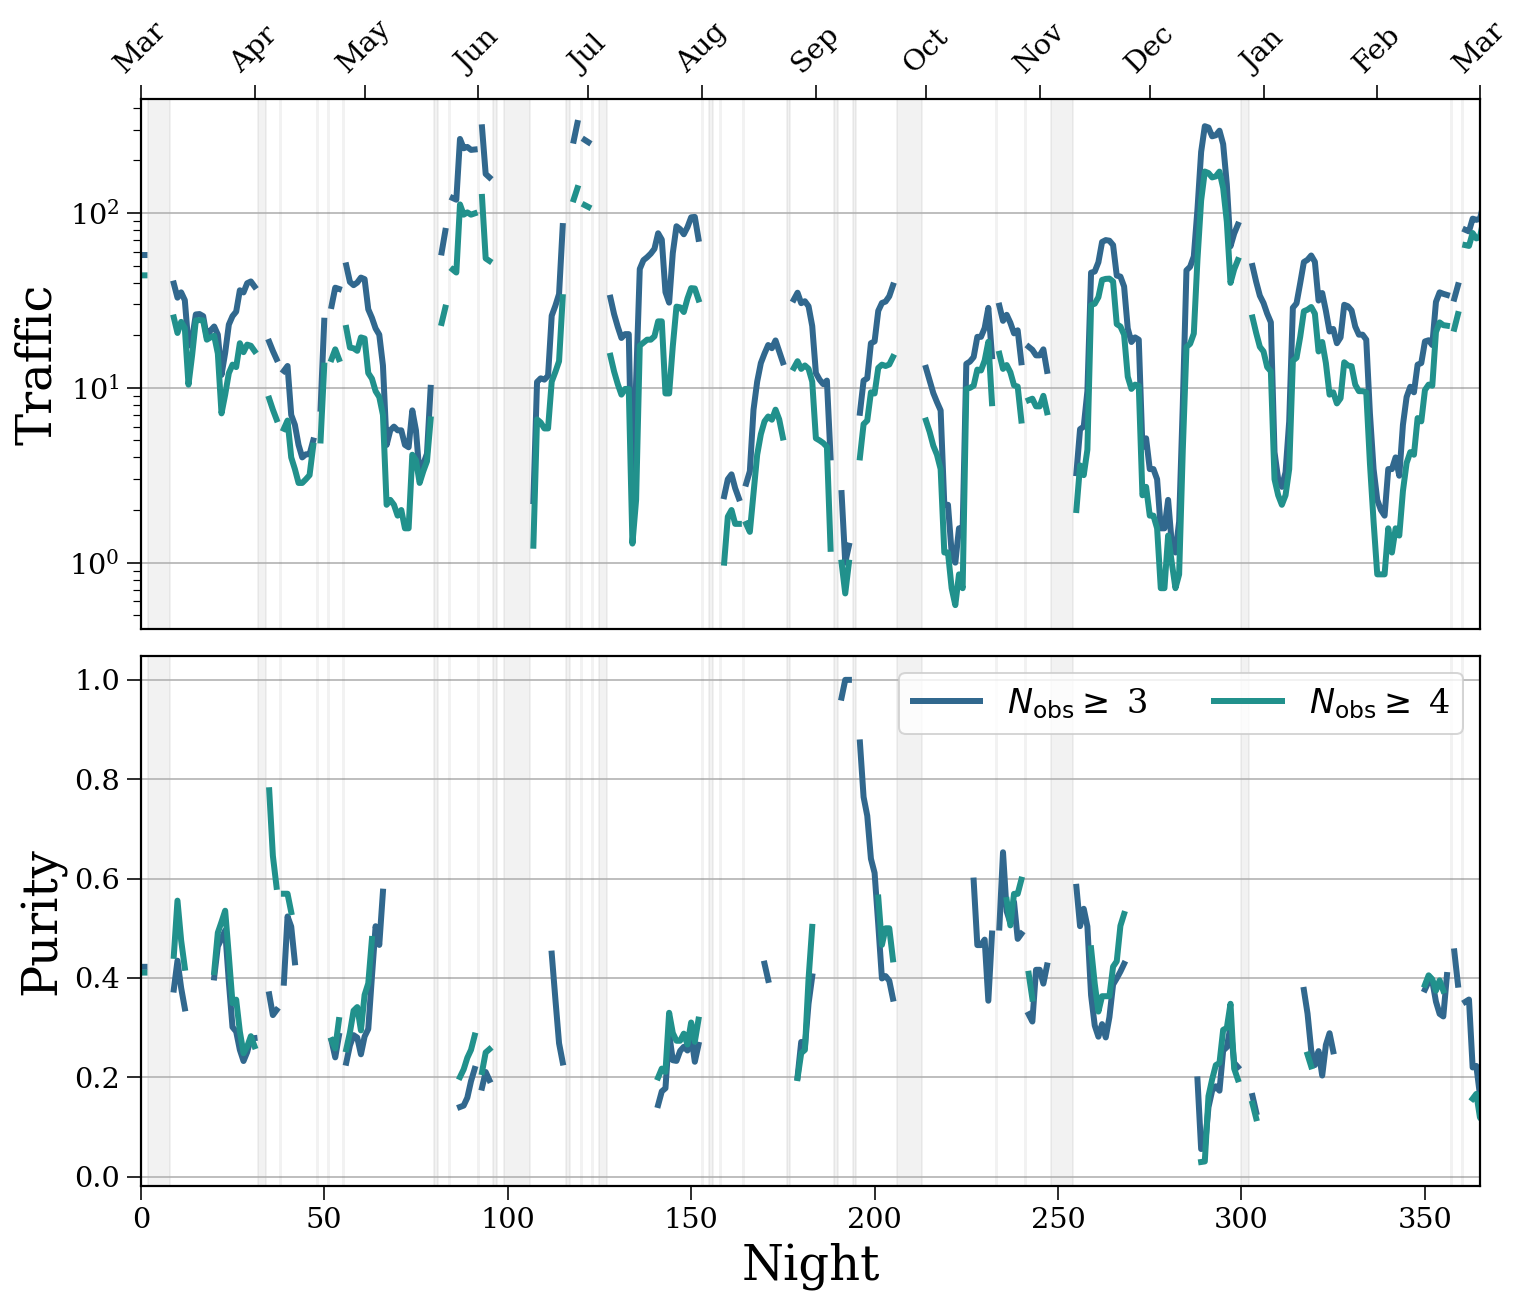
\includegraphics[width=\textwidth]{traffic_purity_unfindable.png}
    \caption{As Figure~\ref{fig:neocp_traffic}, but only including objects that would not be detected by LSST alone. Note the y-scale of the lower panel is now linear.}
    \label{fig:neocp_traffic_unfindable}
\end{figure*}

Overall, it is clear that if we proceed in the same manner as is currently recommended that the NEOCP will not be able to handle the load. We now consider how we could proceed differently.

\subsection{NEOCP without LSST Detections}\label{sec:no_LSST_detections}

LSST will be able to detect and characterise many potential NEOs without any external input. This means that many of the objects submitted to the NEOCP will actual result in wasted follow up time by the community. We assess the magnitude of this effect using the python package \texttt{difi} \citep{difi}. This package calculates which objects are detected by LSST, where a detection is defined as occurring when the same object is observed on at least 3 separate nights within a 15 day window, each with at least 2 observations separated by at most 90 minutes \needcite{}.

In Figure~\ref{fig:neocp_traffic_unfindable}, we repeat Figure~\ref{fig:neocp_traffic}, but now only including objects that would not be detected by LSST alone. This represents a best case scenario in which we had foreknowledge of which observed objects would be detected. In this scenario we see that the traffic from LSST rarely exceeds more than 100 objects and is often only a handful. Similarly the purity is much higher, with an average of around 25\%. We conclude that if we were to know whether an object would be detected by LSST, the load on the NEOCP would remain at manageable levels.

\subsection{Accuracy of LSST detection prediction}
\todo{Demonstrate the efficiency of this method with some plots like fig 3}
\begin{figure*}[htb]
    \centering
    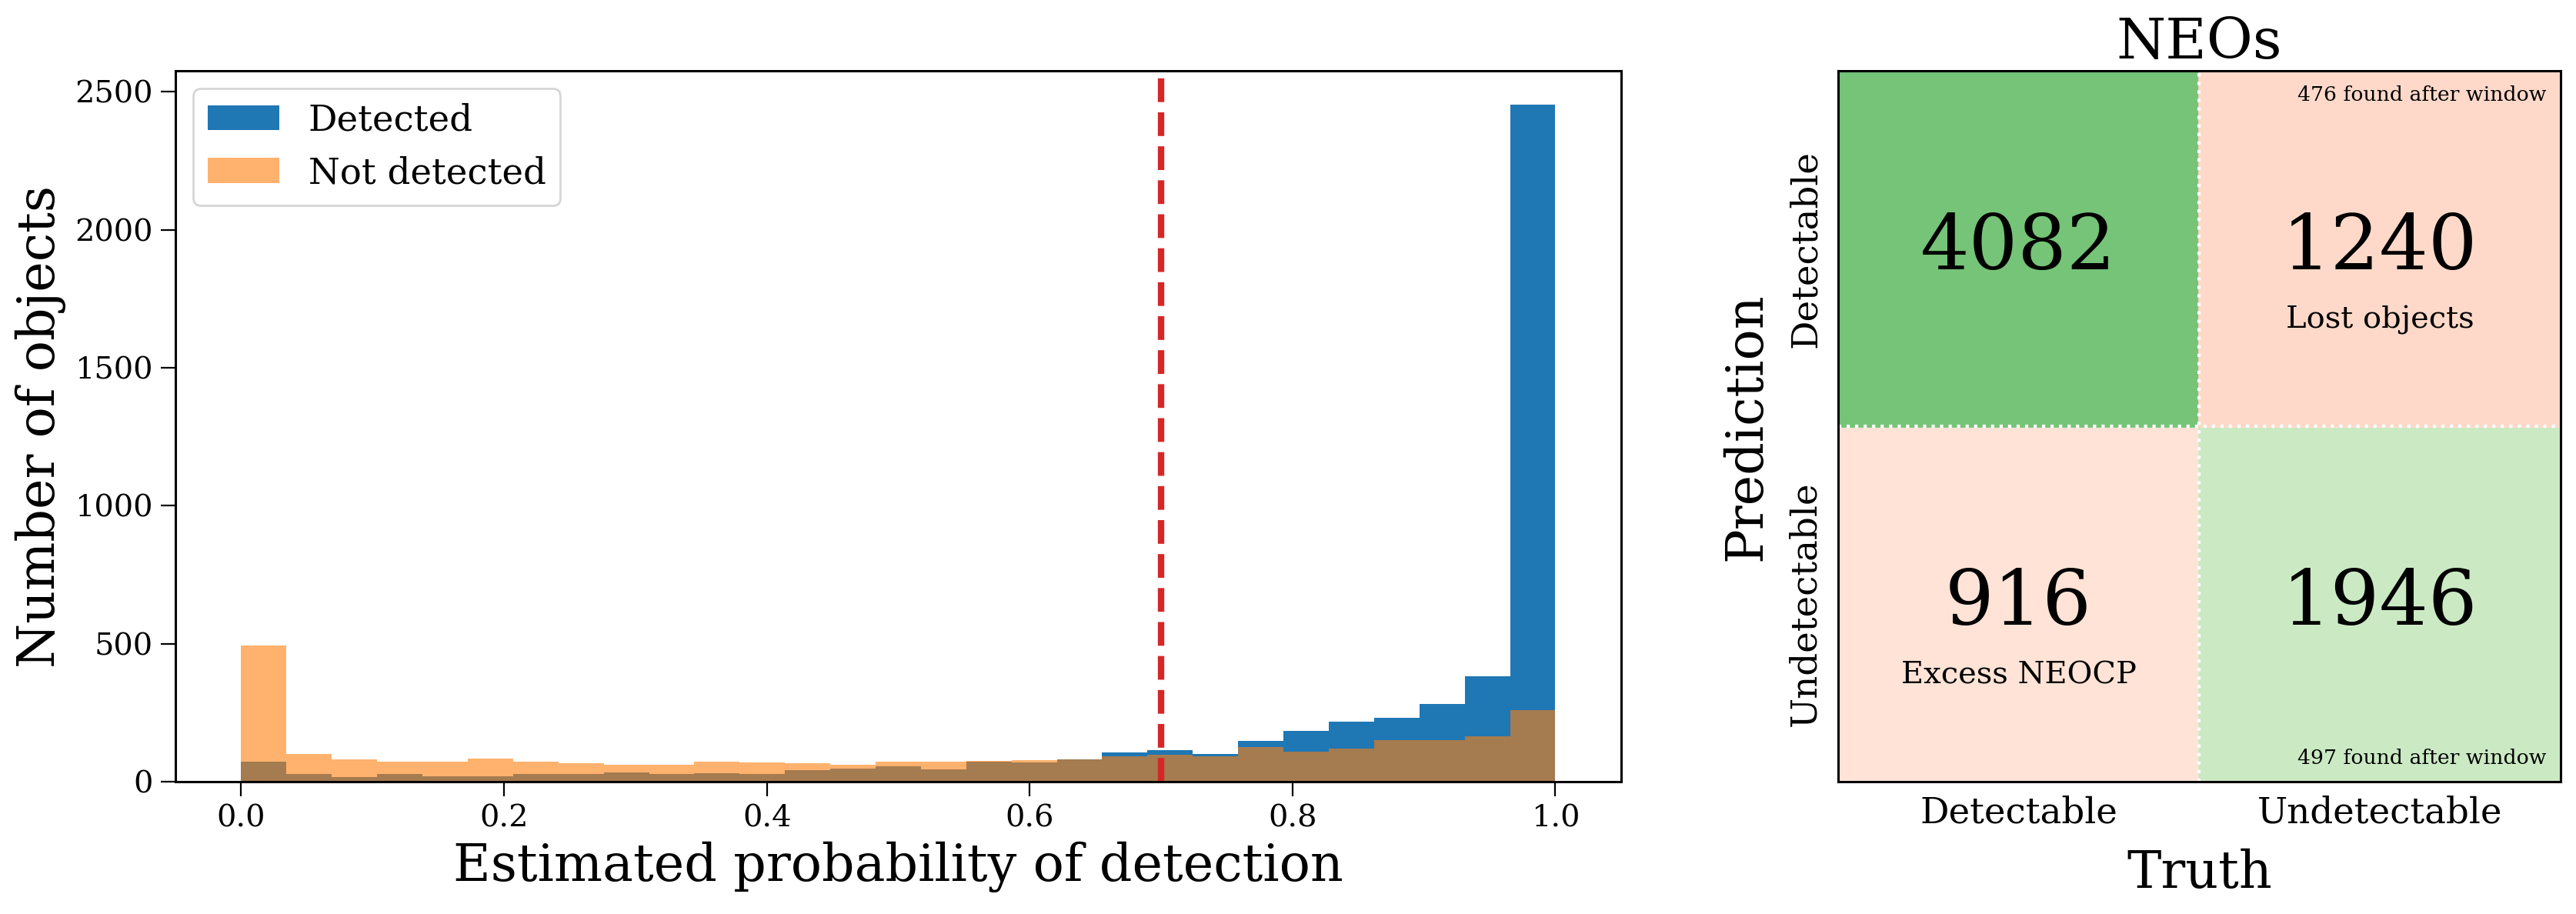
\includegraphics[width=\textwidth]{contingency_neo.png}
    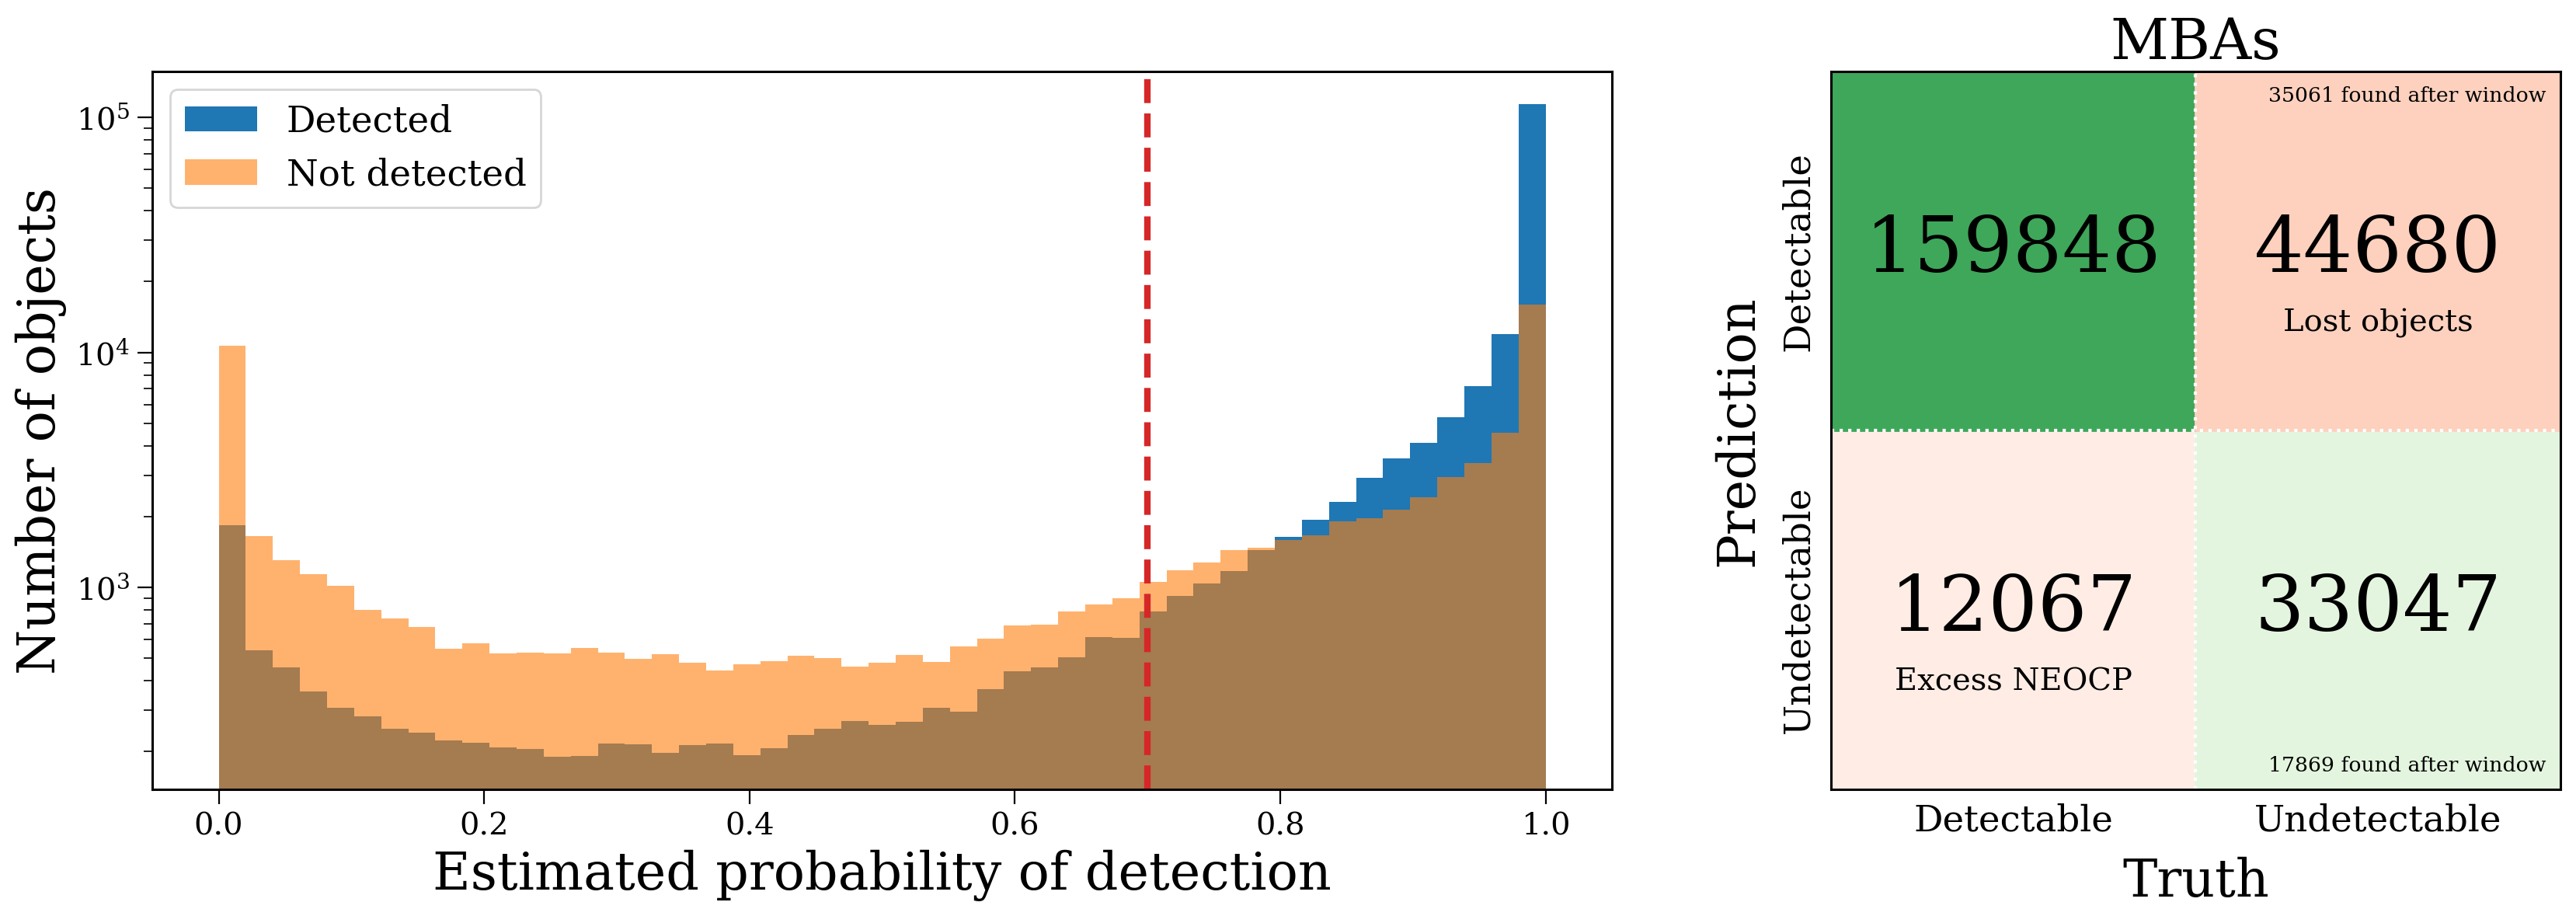
\includegraphics[width=\textwidth]{contingency_mba.png}
    \caption{A demonstration of the prediction algorithm described in Section~\ref{sec:pred_alg} using 1 year of simulated observations for both NEOs (top) and MBAs (bottom). \textbf{Left:} A confusion matrix representing the algorithm's ability to predict the detectability of an object. \textbf{Right:} Probability that an object will be detected within 15 nights, split into a population of objects that are \textit{actually} detected within 15 nights in the simulated observations and a population that are not.}
\end{figure*}

\section{Discussion} \label{sec:discussion}
\subsection{Improving \dig{} algorithm}
\subsection{Await MBA Identification}

\section{Conclusion \& Summary} \label{sec:conclusion}

\todo{Write and summary and spruce up the items below}

\begin{enumerate}
    % \item \textbf{Hybrid Catalogue:} We produce and make available a hybrid catalogue that combines a simulated catalogue \citep{Grav+2011} with detections from \mpco{}. This distributions of the six orbital elements as well as the absolute magnitude in this catalogue are unchanged from \sss{}. The hybrid catalogue can be used to make predictions for LSST that account for prior detections (see Section~\ref{app:hybrid}).
    \item \textbf{NEOCP traffic and purity from LSST:} We show that the traffic (number of objects submitted) and purity (fraction of objects that are NEOs) of the NEOCP will be severely impacted by LSST. We demonstrate that if LSST follows current submission guidelines that the NEOCP would be unable to handle the volume of submissions
    \item \textbf{NEOCP without LSST detections:} We highlight that the traffic and purity of the NEOCP remain at acceptable levels if LSST only submits objects that it won't detect alone
    \item \textbf{LSST detection probability prediction:}
\end{enumerate}

\begin{acknowledgements}
    Acknowledgements
\end{acknowledgements}

\software{\dig{} v0.19.2 \citep{Keys+2019}, \texttt{OpenOrb} \citep{Granvik+2009}, \texttt{difi} \citep{difi}, \texttt{THOR} \citep{Moeyens+2021}, \texttt{Astropy} \citep{astropy:2013, astropy:2018, astropy:2022}, \texttt{astroML} \citep{VanderPlas+2012,VanderPlas+2014}, \texttt{scipy} \citep{Virtanen+2020}}

\bibliographystyle{aasjournal}
\bibliography{paper}{}

\restartappendixnumbering

\allowdisplaybreaks
\appendix

\section{Hybrid Catalogue Pipeline}\label{app:hybrid}
Most studies that make predictions for LSST use a synthetic catalogue of solar system objects that doesn't account for prior observations \needcite{}. In reality, we have already detected more than a million objects in the solar system and this number will continue to grow until LSST comes online. This means that, current predictions of detection rates will be inflated since a fraction of ``new'' detections may already be known. Therefore, for this paper we created ``hybrid'' catalogue that combines a synthetic catalogue with all known observations, whilst keeping the population distributions relatively unchanged.

We created the hybrid catalogue to be dynamic, such that we can run a single pipeline to merge in an updated version of \mpco{} as more objects are discovered in the time until LSST comes online. All code to reproduce this hybrid catalogue is open-source and available on GitHub\footnote{\url{https://github.com/dirac-institute/hybrid_sso_catalogue/tree/main/hybridcat/hybridcat}}.

\subsection{Data preprocessing}
For the synthetic catalogue of the solar system with we use \sss{}, the Pan-STARRS Synthetic Solar System Model \citep[\sss{}][]{Grav+2011}. We merge this synthetic catalogue with the latest version of \mpco{}\footnote{\url{https://minorplanetcenter.net//iau/MPCORB.html}}, a database of all currently known objects. We use \texttt{OpenOrb} \citep{Granvik+2009} to convert both catalogues to Cartesian coordinates and propagate all orbits until the same date.

\subsection{Merging algorithm}
The general idea for the merging algorithm is to inject each object from \mpco{} into \sss{}, replacing objects that are similar to those injected. An object's similarity is determined based on its position, $\va{x}$, velocity, $\va{v}$, and absolute magnitude (size), ${H}$.

We split each catalogue into bins of absolute magnitude linearly spaced from $-2$ to $28$ and perform the merge algorithm on each bin separately. For each bin we build a K-D trees for both catalogues based on the positions ($x, y, z$) of objects. For every \mpco{} object we query the \sss{} tree for the nearest $100$ objects up to a maximum distance of $0.1 \unit{AU}$, excluding any that have already been matched to a different real object. From these remaining nearest neighbours, we select the \sss{} object with the closest velocity as the matched object. If there were no remaining neighbours, either because no synthetic objects were nearby or because all nearby objects had already been matched, then we directly add this real object without replacing a synthetic one.

To complete the merging process, we compile the matched object IDs and delete them from \sss{}. We then add the entirety of \mpco{} to the remaining catalogue, resulting in a hybrid catalogue.

\subsection{Assessing quality of hybrid catalogue}\label{app:hybrid_quality}
It is essential that the underlying distributions of the hybrid catalogue do not differ significantly from \sss{} so that we still accurately reproduce the solar system. In Figure~\ref{fig:hybrid_vs_s3m_dists}, we show the distributions of the absolute magnitude and six orbital elements in both the hybrid catalogue and \sss{}. It is evident that the distributions are essentially identical.

As a further check, we compared \mpco{} to the objects that were removed from \sss{}, since these should have nearly identical distributions. In Figure~\ref{fig:density_compare}, we show a comparison of the densities for the heliocentric $x$ and $y$ and it is clear that these distributions are left unchanged in the hybrid catalogue.
\begin{figure*}[htb]
    \centering
    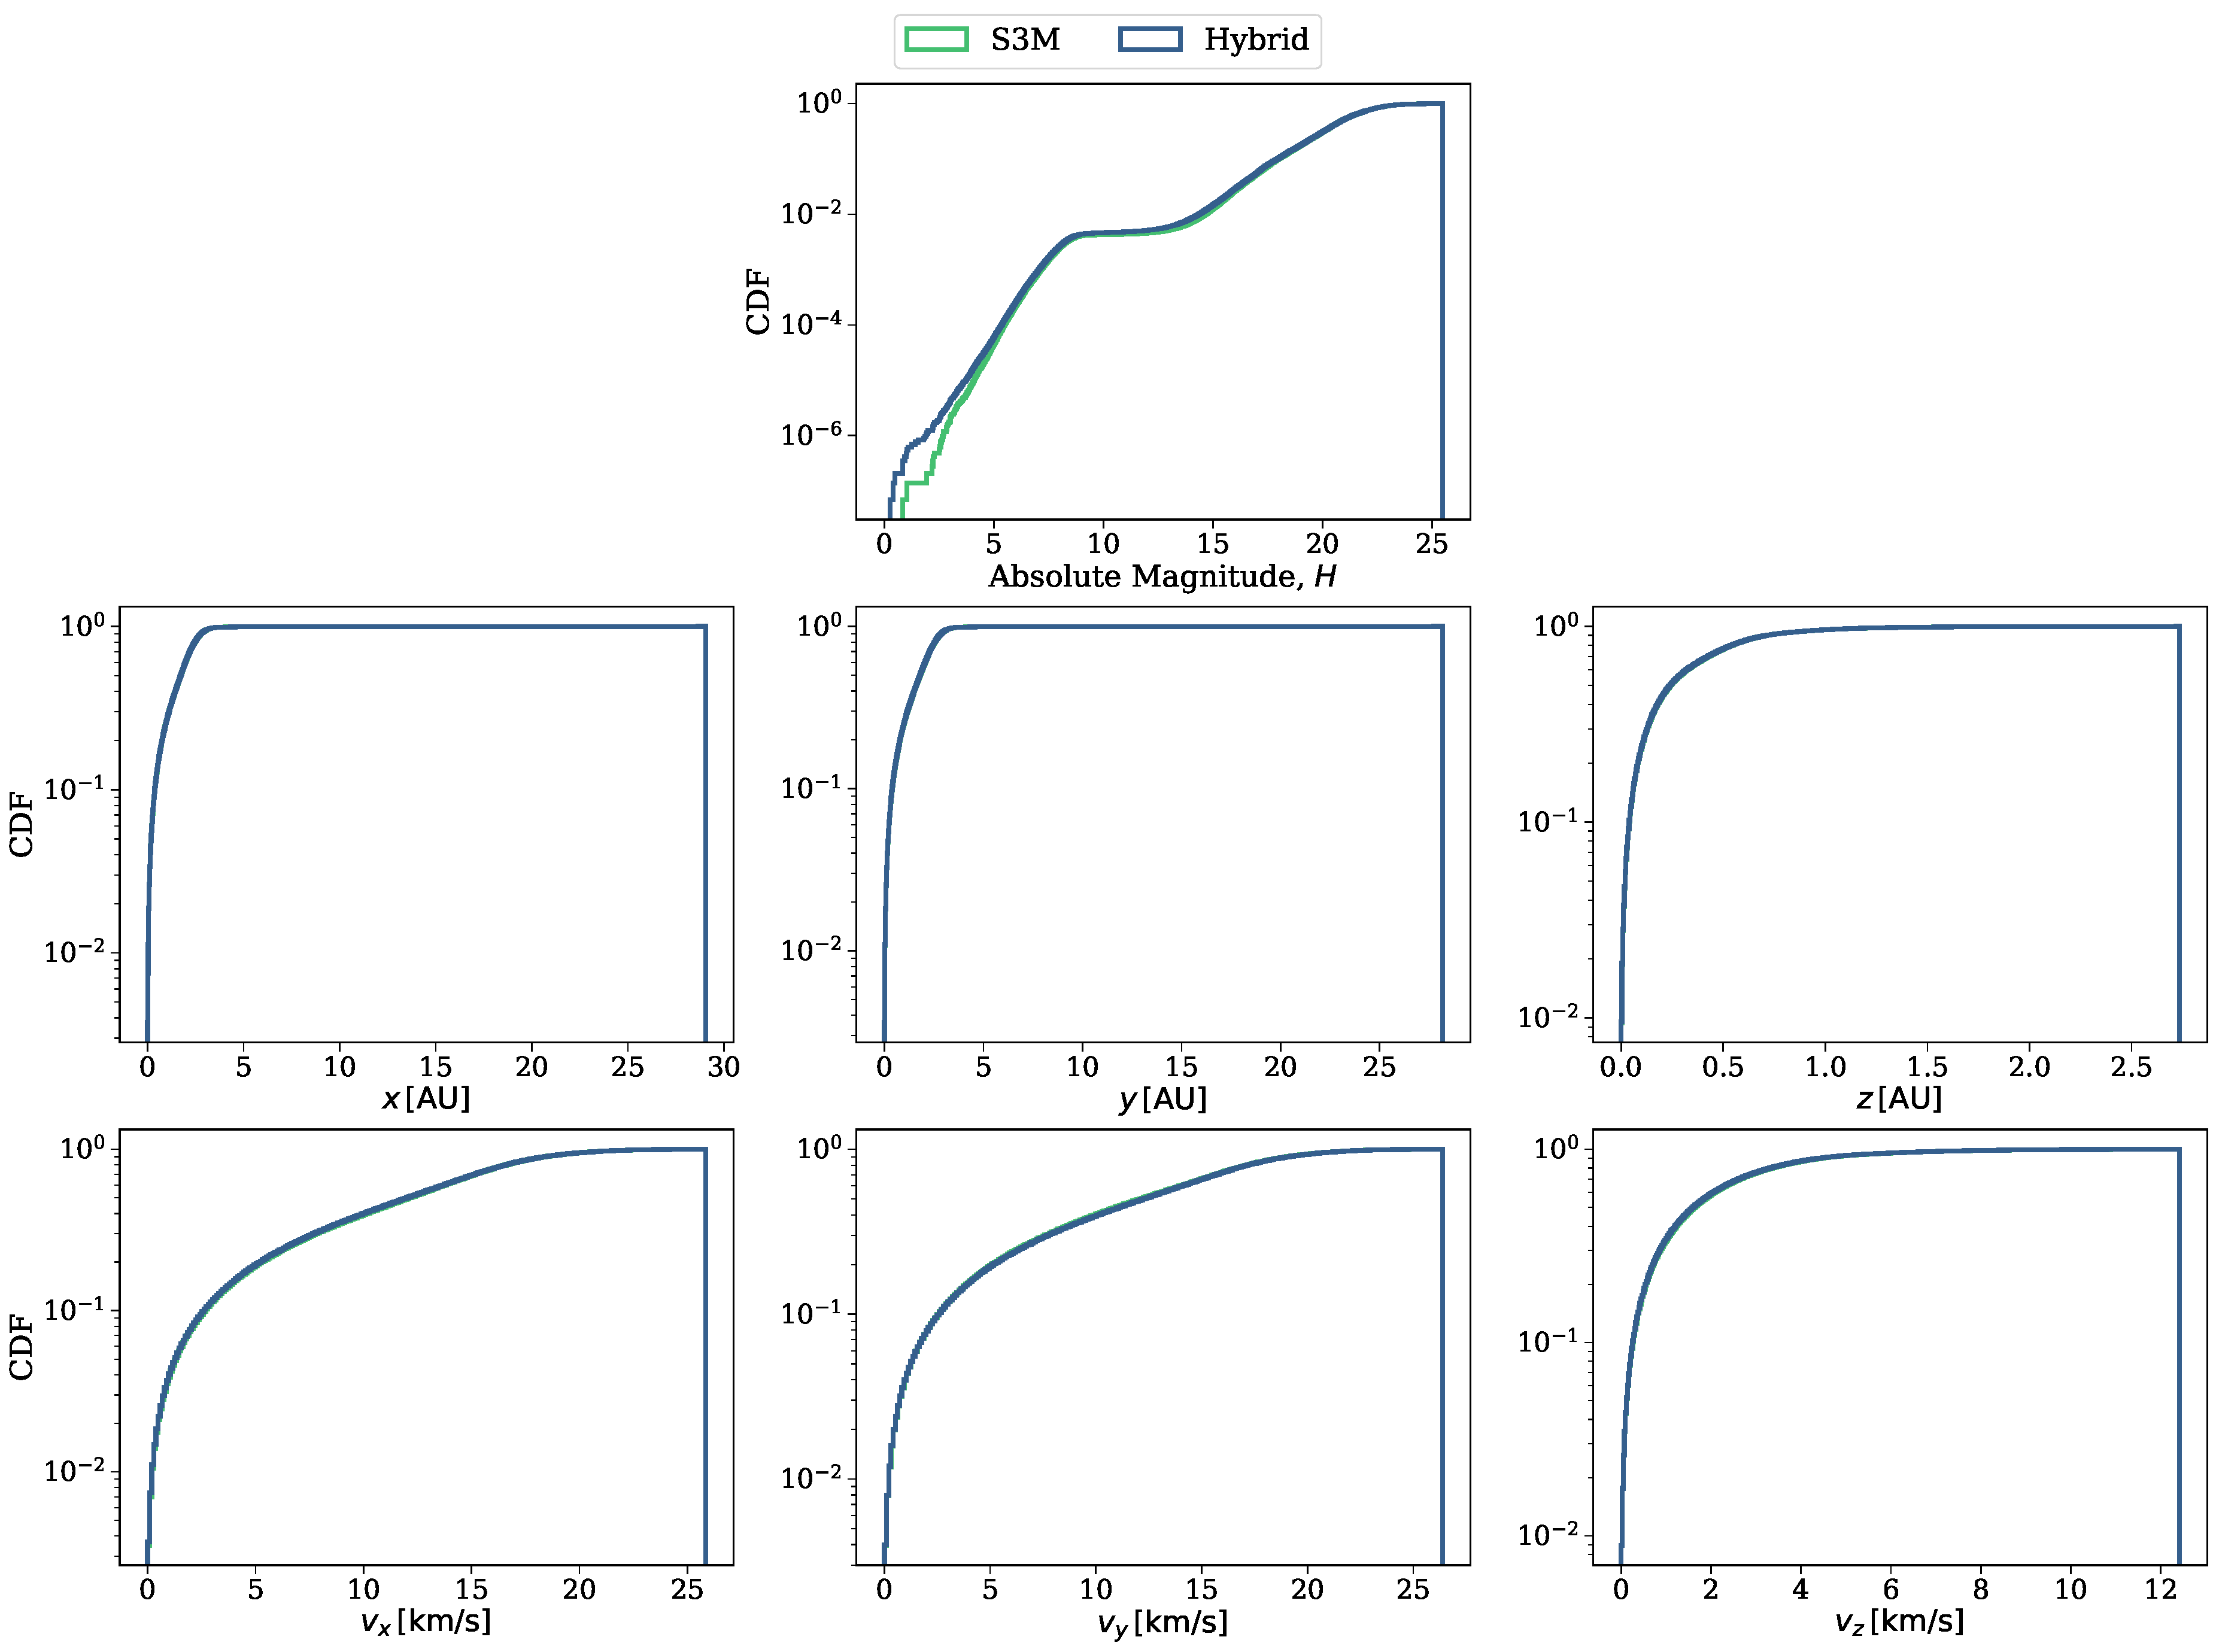
\includegraphics[width=\textwidth]{hybrid_vs_s3m_distributions.pdf}
    \caption{A comparison of the parameter distributions of \sss{} \citep{Grav+2011} and the hybrid catalogue we created.}
    \label{fig:hybrid_vs_s3m_dists}
\end{figure*}
\begin{figure}[htb]
    \centering
    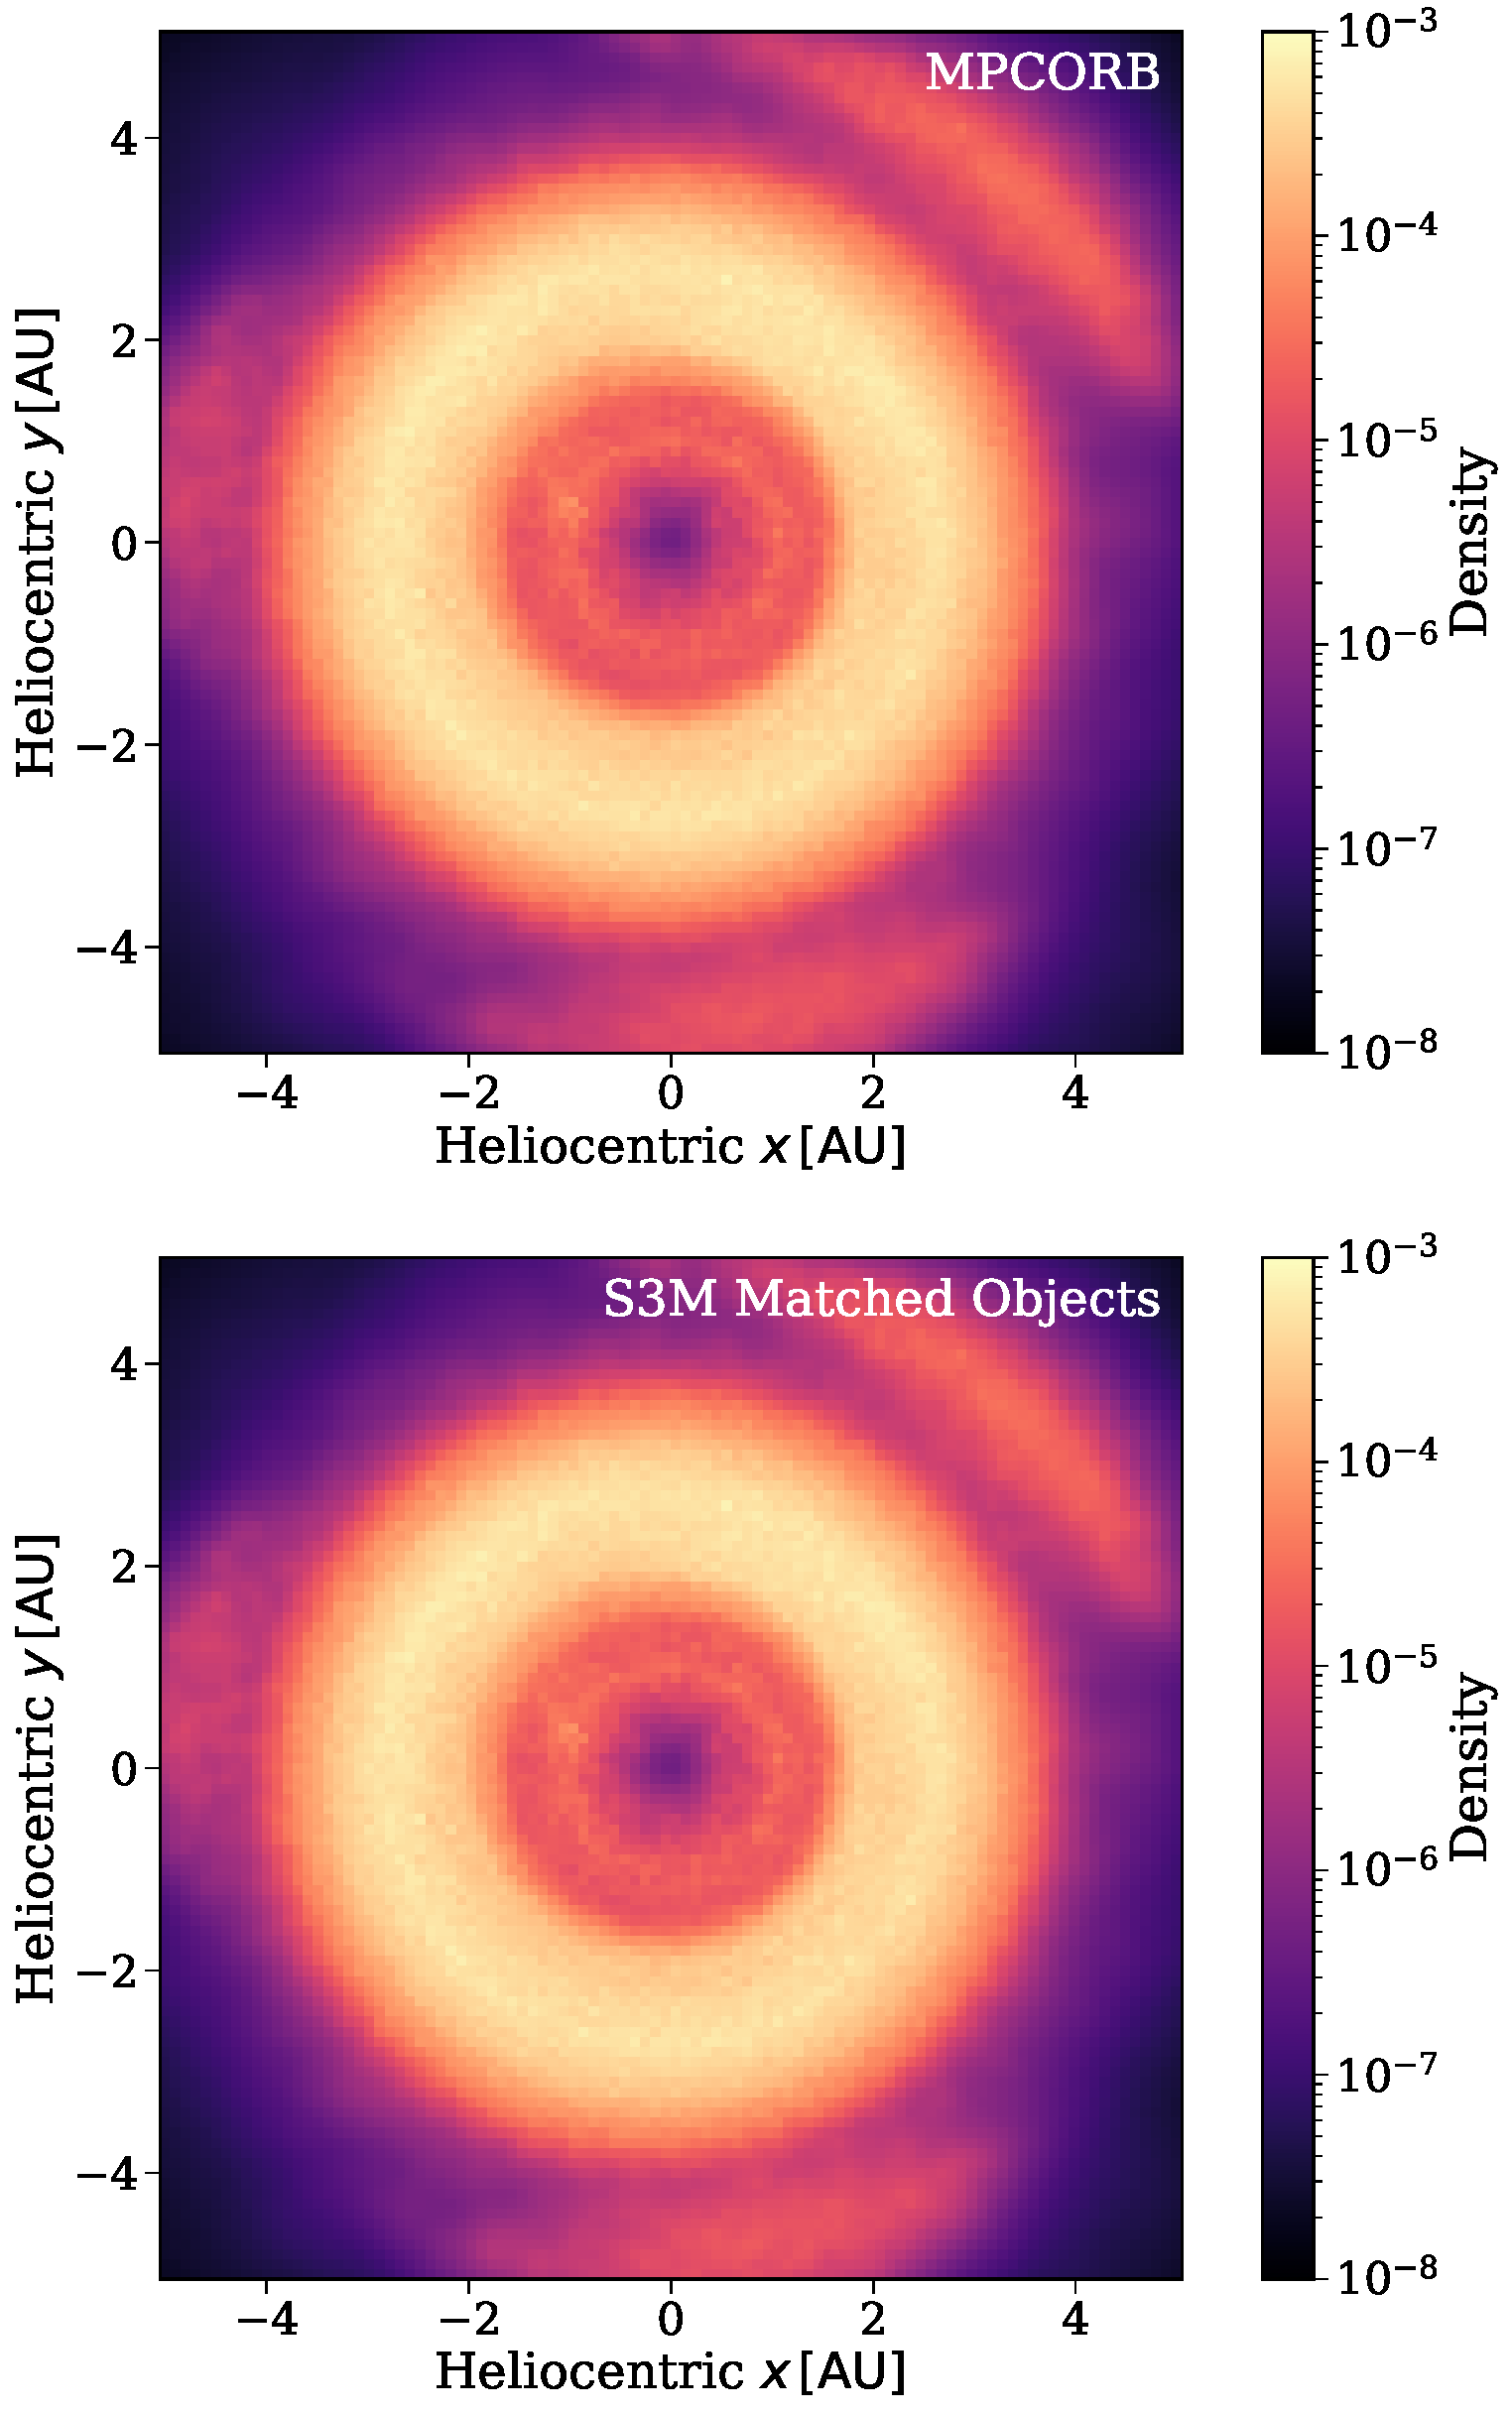
\includegraphics[width=0.48\textwidth]{density_comparisons.pdf}
    \raisebox{0.5\height}{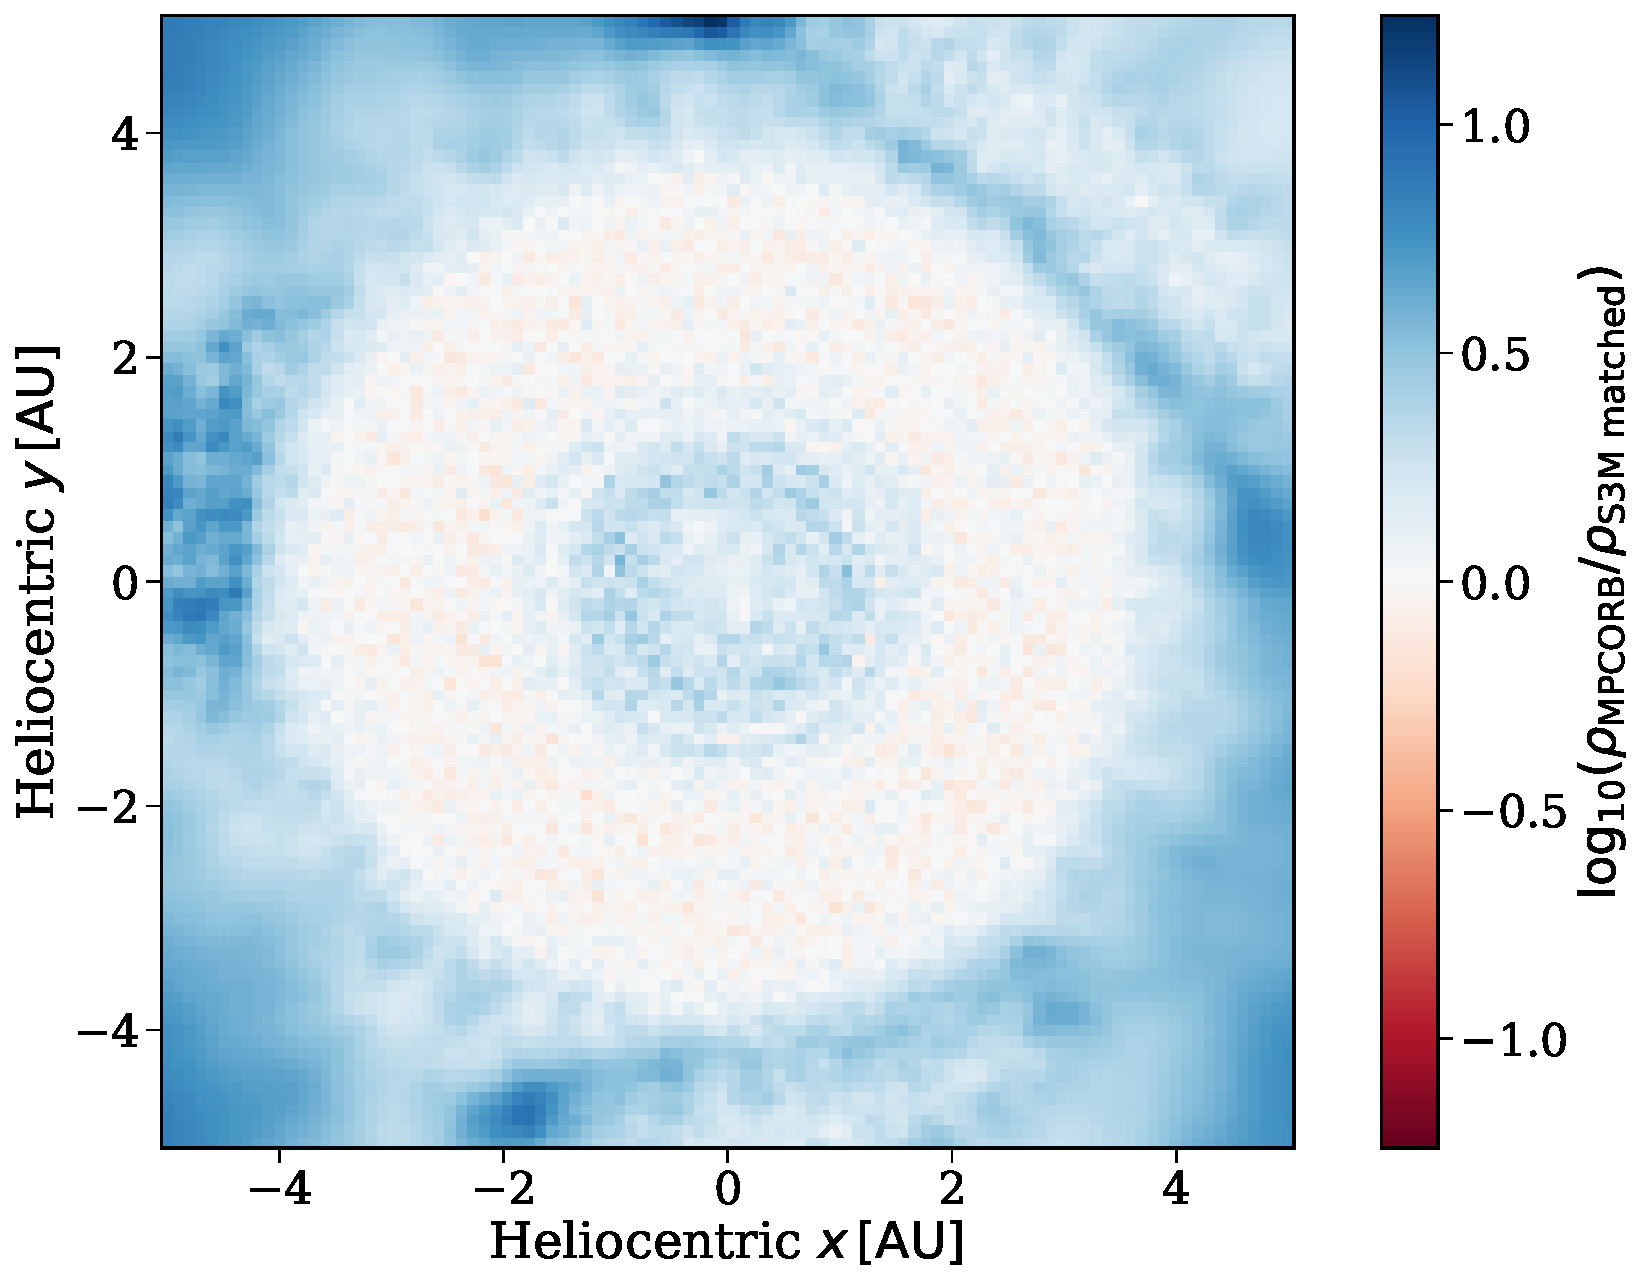
\includegraphics[width=0.48\textwidth]{density_residuals.pdf}}
    \caption{\textbf{Left:} A comparison of the density of \mpco{} objects with those objects that were matched in \sss{} by our hybrid catalogue pipeline. \textbf{Right:} Residuals between the two plots in the left panel.}
    \label{fig:density_compare}
\end{figure}

\end{document}